\JWlone{Implementation}

%#  DATA FORMATS  ##############################################################
\JWltwo{Data Formats}
\label{sec:data-formats}

This chapter will give a rough outline of the formats used to store data between
the various phases of the analysis. The lingua franca for most complex on--disc
formats are the schrieblesque \JWTprotobuf{}. Though, when interfacing with
external software such as \JWTR{}, other formats had to be chosen. The choice in
favor of Protocol Buffers has been made because of \emph{think XML, but
smaller, faster, and simpler} (which is incidentally their  slogan).

%-  shot ids  ------------------------------------------------------------------
\JWlthree{Shot IDs}
\label{sec:shot-ids}

A shot ID (shot identifier) is a string value uniquely identifying a
measuring experiment. More precisely it is a character string containing only a
defined set of ASCII characters. The following regular expression should match
all valid shot IDs: \verb%[a-zA-Z0-9@_-]{1,64}%.

Such shot IDs are always used to associate power and performance event
measurings.


%-  voltage drop data point files  ---------------------------------------------
\JWlthree{Electrical Power Data Point Files}
\label{sec:datapoint-files}

The main matter of the \emph{electrical power data point files} (called
\emph{data point files} for simplicity) is to log the CPU's power consumption by
time. As described in chapter \ref{sec:measuring-setup}, voltage drops are
measured and electrical power and work are calculated later on. This is
why data point files do literally contain voltage drop values by time.
But since the sole reason they exist is to serve as calculation input later on,
they are named after their future meaning.

For practical reasons the representation is designed rather flexible: It
supports arbitrary sampling rates, an arbitrary number of (named) channels and
high--resolution timestamps (up to \SI{1}{\nano\second}).

While researching for this thesis, three channels have been recorded with a
sampling rate of \SI{50}{\kilo\samples\per\second}: \JWchan{CPU}---the CPU's
voltage drops---, \JWchan{BOARD}---the motherboard's voltage drops (unused)---
and \JWchan{TRIGGER}---the trigger wire used to mark the periods of time the
other machine counts performance events.

The data point files are also one notable exception of the \emph{Protocol
Buffers for everything} principle in this work. Protocol Buffers were not
designed to handle large messages but to serve as individual messages
\emph{within} a large data set \cite{google11pbtechniques}. So (as you can see
in appendix \ref{sec:fmt:datapoints}) small Protocol Buffer messages are
streamed one after another. The size of one of these chunks is not specified.
Usually one makes up a chunk when he receives one from a measuring device. The
rule of thumb is: Make them as large as practical, but not too large since we
only record one time stamp per chunk. The data points inside each chunk are
considered as distributed equally.


%-  performance counter files  -------------------------------------------------
\JWlthree{Counter Files}
\label{sec:counter-files}

The \emph{counter files} are used to save the performance event counter values
after the completion of one measuring experiment. Having the performance event
counter values and the electrical work of one measuring experiment is an
essential part toward calculating an energy model (see chapter
\ref{sec:towards-the-model}). The match of corresponding data point files
(chapter \ref{sec:datapoint-files}) and counter files is done using the shot ID
(chapter \ref{sec:shot-ids}).

The counter files' on--disc representation is---except for some magic bytes---
a Protocol Buffers--only format. For the technical definition see appendix
\ref{sec:pb:counter-files}.


%-  work files  ----------------------------------------------------------------
\JWlthree{Work Files}
\label{sec:work-files}

The content of the work files is just the electrical work of a certain
measuring experiment in Joule. The file format is the ASCII representation of a
floating point value followed by optional garbage (separated by an ASCII space
or newline). In contrast to the other file formats, the work file's file names
have to match the following format: \verb%work_<SHOT-ID>_.work% (e.\,g.\ 
\verb%work_SPEC-gcc@2011-08-31_16-07-46.work%).

The following listing shows a valid work file:

\begin{lstlisting}[style=Shell]
$ hexdump -C work_SPEC-gcc@2011-08-31_16-07-46.work
0000  37 34 2e 30 31 35 32 35  36 0a   |74.015256.|
000a
\end{lstlisting}




%#  TOOLS  #####################################################################
\JWltwo{Software Tools}
\label{sec:tools}

Since the building of a reasonable energy model is not an easy task, numerous
tools have been used. Most software was developed specifically for the purpose
of this study thesis. All of it is open--sourced and available on
\JWnamedlink{https://github.com/weissi/studienarbeit}{GitHub}
(\JWlink{https://github.com/weissi/studienarbeit}).

This chapter will give an overview of the software used, both standard software
and tools developed specifically.


%-  standard software  ---------------------------------------------------------
\JWlthree{Standard Software}
\label{sec:standard-software}

\begin{itemize}

\item \JWTLprotobuf{} --- for saving and loading of all kinds of data

\item
\JWnamedlink{http://hackage.haskell.org/cgi-bin/hackage-scripts/package/protocol-buffers}
{\JWpn{protocol-buffers}} --- for parsing \JWTprotobuf{} files and generating
code in Haskell

\item \JWnamedlink{http://code.google.com/p/protobuf-c/}{\JWpn{protobuf-c}} ---
for parsing Protocol Buffer files in generating code in C

\item \JWTLR{} --- for statistical computations

\item \JWnamedlink{http://cran.r-project.org/web/packages/leaps/}{\JWpn{leaps}}
--- a \JWTR{} library for regression subset selection (to minimize the set of
available performance counters)

\item
\JWnamedlink{http://stat.ethz.ch/R-manual/R-devel/library/stats/html/lm.html}
{\JWpn{lm}} --- a \JWTR{} library to fit linear models

\item \JWnamedlink{http://perfmon2.sourceforge.net/docs_v4.html}
{\JWpn{libpfm4}} --- for reading the performance counters from userspace

\item \JWTLnidaqmxbase{} --- for interfacing \JWPni

\item \JWnamedlink{http://www.haskell.org/ghc}{\JWpn{Glasgow Haskell Compiler}}

\item \JWnamedlink{http://kernel.org}{\JWpn{Linux Kernel}}

\item numerous \JWnamedlink{http://gnu.org}{\JWpn{GNU}} tools

\end{itemize}


%-  special developments  ------------------------------------------------------
\JWlthree{Special Developments}
\label{sec:special-developments}


\JWlfour{\JWTlibdp{}}

\JWTlibdp{} is responsible for loading and saving the measured data points from
and to the data point files (see chapter \ref{sec:datapoint-files}). Its API is
straight forward and the library is able to handle arbitrarily large files. The
API can be found in \JWpath{libdatapoints/datapoints.h}.


\JWlfour{\JWTdd{}}

\JWTdd{} is the tool used to dump the measuring data to data point files (see
chapter \ref{sec:datapoint-files}). It currently records the three channels
\JWchan{CPU}, \JWchan{BOARD} and \JWchan{TRIGGER} with a sampling rate of
\SI{50}{\kilo\samples\per\second} using \JWTnidaqmxbase{} (see chapters
\ref{sec:measuring-device} and \ref{sec:standard-software}) to a file.
Again, the usage is quite simple and straight forward:

\begin{lstlisting}[style=Shell]
datadump out.dpts my-shot-id
\end{lstlisting}

The example saves the measuring experiment \texttt{my-shot-id}'s data to the
file \JWpath{out.dpts}. The record runs until a \texttt{SIGINT} signal is
caught. Optionally a third parameter representing the desired maximal running
time in seconds is supported.


\JWlfour{\JWTfcw{}}

\JWTfcw{} can calculate the electrical work from data point files quick\-ly. As
explained in chapter \ref{sec:calc-work} it calculates and integrates the
instantaneous power to electrical work. But since discrete data is obtained by
sampling (see chapter \ref{sec:measuring-setup}), calculating the electrical
work is easy and fast:

\begin{eqnarray}
P(t) & = & \frac{12V * U_R(t)}{R} \\
W & = & \int_{t_0}^{t_{max}} P(t)dt = \sum_{i=1}^{max}P(t_i)*(t_i-t_{i-1})
\end{eqnarray}

The following example illustrates the usage of \JWTfcw{}:

\begin{lstlisting}[style=Shell]
fastcalcwork captured-17:15:00.dpts CPU 0.01 TRIGGER
\end{lstlisting}

Using the command line above, \JWTfcw{} will calculate the electrical work with
a measuring resistor of \SI{0.01}{\ohm}. The measured data points will be taken
from column \JWchan{CPU}, the analog trigger's value (see chapter
\ref{sec:measuring-setup}) from \JWchan{TRIGGER}.


\JWlfour{\JWTde{}}

\JWTde{} exports data point files (see chapter \ref{sec:datapoint-files}) to
\JWTR{}'s \texttt{read.table} format \cite{r11data}. This format is less
efficient and contains only parts of the information but enables user to exploit
\JWTR{}'s excellent analysis and plotting abilities.


\JWlfour{\JWTdc{}}

\JWTdc{} is a tool for retrieving the performance event's counter values on the
target machine. Giving it a set of performance events and a command to execute,
it will record the events while the task is running. It always works
system--widely and saves values by counter and by CPU enabled. Along the way it
also controls the trigger wire. The trigger is crucial to match the time
intervals intervals for counting performance events and measuring electrical
power.

A working example executing \JWpath{/bin/ls} and counting
\JWctrCLK{} and \JWctrINST{} along the way follows:

\begin{lstlisting}[style=Shell]
dumpcounters -e CPU_CLK_UNHALTED,INST_RETIRED \
             -o ls_clock-cycles_inst-retired.ctrs \
             -r /bin/ls
\end{lstlisting}

After the execution, the file \JWpath{ls_clock-cycles_inst-retired.ctrs} will
contain the performance event counter values. The file format is described in
chapter \ref{sec:counter-files}.


\JWlfour{\JWTcbs{} suite}

\JWTcbs{} suite is a front end and a very small library making it easy to write
and use microbenchmarks.  It is primarily meant to stress individual performance
event counters, hence its name. Working samples can be found in the directory
\JWpath{ctrbenchmark/benchlets/}.


\JWlfour{\JWTbsle}

\JWTbsle{} is a \JWnamedlink{http://haskell.org}{Haskell} program which is able
to \emph{build} the \emph{s}ystem of \emph{l}inear \emph{e}quations. It takes
several counter files (chapter \ref{sec:counter-files}) and the corresponding
work files (\ref{sec:work-files}) as input and outputs a system of linear
equations.

Given that \JWTR{} was always used to post-process the results of \JWTbsle{}
it is obvious that, again, \JWTR's \texttt{read.table} \cite{r11data} format is
outputted. Building a system of linear equations and solving it in \JWTR{}
works as the following example shows:

\begin{lstlisting}[style=Shell]
$ buildsle *.work *.ctrs > /tmp/sle.rtab
BuildSLE, Copyright (C)2011, Johannes Weiss
[...]
Processed work files: 500
[...]
$ R

R version 2.12.1 (2010-12-16)
[...]
> sle <- read.table('/tmp/sle.rtab', header=TRUE)
> m <- lm(WORK~., data=sle)
\end{lstlisting}


\JWlfour{high--level scripts}

So far, there are several simple tools for simple tasks. To compose the ensemble
many of them have to be invoked correctly with each other. Since this is not a
trivial task, some high--level scripts have been developed, most notably
\JWpath{scripts/measure-n-counters-m-benchmarks.sh} and \JWTdomeasuring{}.  The
former script can control records of many benchmarks with a fixed (chapter
\ref{sec:final-model}), rotational (chapter \ref{sec:finding-useful-subset}) or
incremental (chapter \ref{sec:overhead}) set of performance event counters; the
latter automates the following steps as shown in the example below:

\begin{enumerate}

\item Check if no other measuring experiment is currently running.

\item Check that \JWPni{} is connected.

\item Check that the login to the remote machine \texttt{i30pc59} works
password--less and the remote user is allowed to use \JWpn{sudo}.

\item Locally and remotely build the needed software tools.

\item Locally start \JWTdd{}, remotely launch \JWpath{/bin/ls} using \JWTdc{}.
The counted performance events are \JWctrCLK{} and \JWctrINST{}.

\item Wait until \JWpath{/bin/ls} has terminated and then stop \JWTdd{}.

\item Calculate the electrical work using \JWTfcw{}.

\item Save the data dump file, the counter file and the work file under the
directory \JWpath{/tmp/demo-shot}. The shot--id is
\texttt{demo-\-shot\-@2001-\-09-\-09\_\-15-\-41-\-32}.

\end{enumerate}

\begin{lstlisting}[style=Shell]
$ do_measuring.sh -f \
                  -s 2011-09-09_15-41-32 \
                  -p demo-shot \
                  -o /tmp/demo-shot \
                  i30pc59 \
                  'CPU_CLK_UNHALTED,INST_RETIRED' \
                  /bin/ls
No other 'datadump' running: OK
Checking if NI device 3923:7272 is plugged: OK
Testing password-free SSH: OK
Testing password-free sudo: OK
Building: OK
Remote building: OK
INFO: logfile is '/tmp/measuring_log_[...].log'
Waiting for sloooow NI call (e.g. 29s) [...].OK[...]
Writing remote script: OK
Running remote benchmark: OK (time=1)
INFO: remote log is '/tmp/remote-[...].log'
Telling datadump to stop (SIGINT): OK
Waiting for dump process (23472) to finish ....OK
Calculating work to 'work_[...].work' OK
Doing transformation

GREAT SUCCESS, EVERYTHING WENT FINE :-)
\end{lstlisting}




%#  TOWARD THE ENERGY MODEL  ###################################################
\JWltwo{Toward the Energy Model}
\label{sec:towards-the-model}

In this chapter a description of the steps toward the final energy model(s) is
given.


%-  BENCHMARKS  ----------------------------------------------------------------
\JWlthree{The Set of Benchmarks}
\label{sec:benchmarks}

The first step toward the energy model is to choose a good set of benchmarks.
The benchmarks should stress different parts of the CPU and should collectively
stress all parts and units of the CPU. As chapter \ref{sec:restrictions} states
some units have been deliberately excluded in this work. The benchmarks should
therefore avoid the excluded units because their results would have bad
consequences on the final model.

The benchmark choice fell to the \JWTLspec{} suite, the memory bandwidth
benchmark \JWTLstream{} a benchmark provoking many branch mispredictions
and an ALU stress benchmark.

For the multi--core tests, different instances of these benchmarks have been
pinned to each core and were therefore running simultaneously.


%-  SUBSET OF USEFUL COUNTERS  -------------------------------------------------
\JWlthree{Finding a useful Subset of Events}
\label{sec:finding-useful-subset}

Because of the symmetric architecture of the CPU (see chapter
\ref{sec:sandy-bridge}) the final subset of events in the model has been
gathered using only one enabled core of the CPU. The other cores have been
disabled using the BIOS.

To model the baseline energy of a core (the energy consumed when no performance
event is triggered), one pseudo--event per core (modeling the time it is
enabled) has been added. These events fall in the group of the \emph{global
events} (see chapter \ref{sec:model-properties}). A core can only be enabled or
disabled when the machine gets (re)booted. Therefore each of these
pseudo--events is either $0$ (core \emph{disabled}) or is equal to the entire
running time of a benchmark (core \emph{enabled}).

The general methodology has already been described in chapter
\ref{sec:min-events}.  First the performance events were randomly
distributed in disjoint groups of eight events which is the maximal number of
performance events the CPU can count simultaneously (see chapter
\ref{sec:sandy-bridge}). Thereafter, for each group of events all benchmarks
have been executed consecutively. Then all the runs of each benchmark were
considered as one run recording all available events. Since the electrical
work consumed and the running time was recorded for each run of its own they
were averaged per benchmark. Because the maximal relative standard deviation
was always below 4\%, there was no danger of averaging them.

The result was considered as one huge system of linear equations and the best
subset of events was chosen using \JWTleaps{}. The events \JWctrCLK{} ($=$
\JWctr{CPU\_\-CLK\_\-UNHALTED.\-THREAD} $\propto$
\JWctr{CPU\_\-CLK\_\-UNHALTED.\-REF\_\-TSC}) and \JWctrINST{} ($=$
\JWctr{INST\_\-RETIRED.\-ANY}) are counted using fixed counters (see chapter
\ref{sec:pmu}) and were therefore forced into the model. Except the two fixed
counters, \JWTleaps{} has been configured to find the best model for eight
counters.

Appendix \ref{appendix:chosen-events} describes the events forming the energy
model presented in this paper.


%-  FINAL MODEL  ---------------------------------------------------------------
\JWlthree{Final Energy Model}
\label{sec:final-model}

\begin{figure}
  \centering
    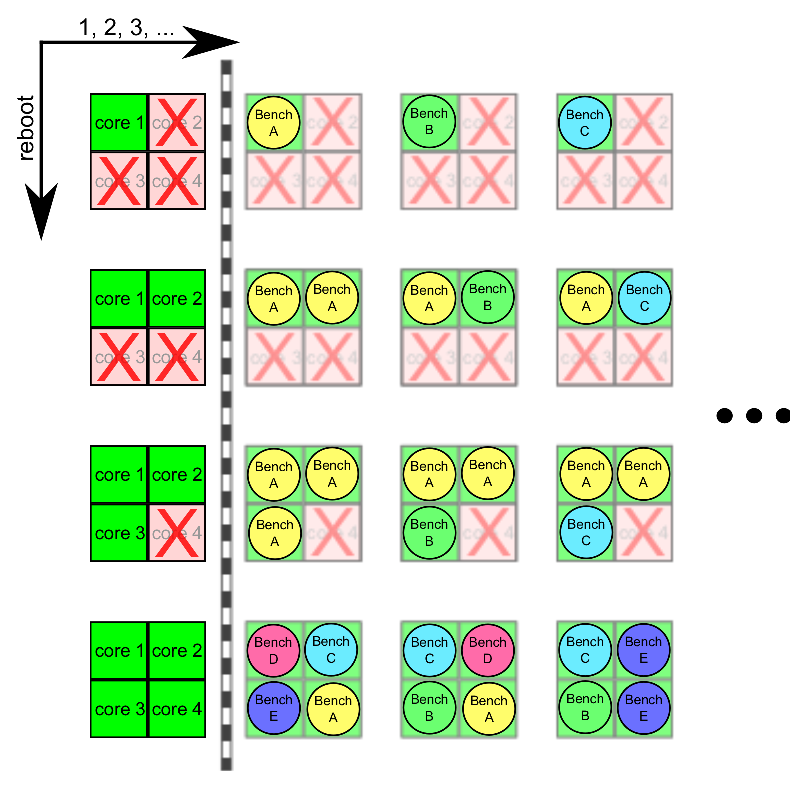
\includegraphics[width=\textwidth]{fig/run-benchmarks.eps}
  \caption{Data acquisition by running benchmark permutations}
  \label{fig:run-benchmarks}
\end{figure}

After the event selection process, suitable energy weights for the
(pseudo--)event had to be found. To find these, the benchmarks runs were
repeated---once again on a single core but recording all of the final events in
one shot. Thereafter all reasonable permutations for two and three cores and 500
random permutations for all four cores have been generated. All in all over 3000
different benchmark runs have been recorded. The way the benchmark runs were
recorded is illustrated in figure \ref{fig:run-benchmarks}. It was necessary to
always reboot and reconfigure the machine because the number of active cores
cannot be changed at runtime. The \JWpn{taskset}\cite{man:taskset} utility has
been used to pin the benchmark processes to their target core.

To train the model only about 50 well chosen benchmark runs were used,
iteratively adding adequate sample runs when weaknesses of the model have been
discovered. To evaluate the model (chapter \ref{sec:evaluation}) the whole set
was used.

Presumably due to the symmetric architecture of the CPU, the events' energy
weights proved to be similar on all cores. Hence, the model's general form could
be simplified. Consequently the function $w_c$ is not anymore parametrized by
core. The following equation shows the new form, identifiers as in chapter
\ref{sec:model-properties}.

\begin{equation}
W(t_0, t_e) = \sum\limits_{i=1}^{n_g} c_g(i, t_0, t_e) w_g(i) +
\sum\limits_{k=1}^{n_e} w_e(k) \sum\limits_{j=1}^{n_c}
c_e(j, k, t_0, t_e)
\end{equation}

The following table shows the energy weights which form the functions $w_c$ and
$w_g$. $c_g$ and $c_e$ are the system's live data, available from the PMU (via
\JWTlibpfm{}). When running live on a system, the parameters $t_0$ and $t_e$
result from the sampling process: $t_0$ is the point in time of the last sample,
$t_e$ is ``now''. The functions' values are then obtained by the performance
event counter's difference between the last and the current sample. Obviously,
$c_g$ and $c_e$ are partial functions in reality: They are only defined if $t_0$
matches the time of the last sample and $t_e$ the time of the current sample.
The formula above and the weights below represent the energy model presented in
this thesis. That is enough to estimate the electrical power the CPU consumed in
selectable sampling intervals.

\begin{tabular}{l r r}

(pseudo--)Event &
Energy&
Maximal Frequency\\
& Weight & compared to\\
& ($w_c$ and $w_g$) & \JWctr{CPU\_CLK\_UNHALTED} \\

\hline
\textit{time core 1 is enabled} [\si{\nano\second}] &
\SI{7.122}{\nano\joule} &
$\infty$ \\

\textit{time core 2 is enabled} [\si{\nano\second}] &
\SI{1.486}{\nano\joule} &
$\infty$ \\

\textit{time core 3 is enabled} [\si{\nano\second}] &
\SI{1.591}{\nano\joule} &
$\infty$ \\

\textit{time core 4 is enabled} [\si{\nano\second}] &
\SI{2.350}{\nano\joule} &
$\infty$ \\

\hline

\JWctr{INST\_RETIRED} &
\SI{-0.224}{\nano\joule} &
245.01\% \\

\JWctr{CPU\_CLK\_UNHALTED} &
\SI{4.546}{\nano\joule} &
100.00\% \\

\JWctr{LD\_BLOCKS:DATA\_UNKNOWN} &
\SI{-6.281}{\nano\joule} &
83.28\% \\

\JWctr{LD\_BLOCKS:ALL\_BLOCK} &
\SI{5.504}{\nano\joule} &
83.28\% \\

\JWctr{UOPS\_DISPATCHED:STALL\_CYCLES} &
\SI{-2.508}{\nano\joule} &
72.44\% \\

\JWctr{ILD\_STALL:IQ\_FULL} &
\SI{-1.425}{\nano\joule} &
18.17\% \\

\JWctr{DSB2MITE\_SWITCHES} &
\SI{-5.972}{\nano\joule} &
5.31\% \\

\JWctr{DSB\_FILL:ALL\_CANCEL} &
\SI{64.249}{\nano\joule} &
2.60\% \\

\JWctr{L2\_RQSTS:PF\_HIT} &
\SI{-22.837}{\nano\joule} &
1.23\% \\

\JWctr{BR\_INST\_RETIRED:FAR\_BRANCH}  &
\SI{-18031.295}{\nano\joule} &
0.05\% \\

\hline

\end{tabular}


% vim: set spell spelllang=en_us fileencoding=utf8 : syntax spell toplevel :
